\chapter{The distance to rho, family by family}\label{ch:distance}

This chapter gives, for each curve family, the current distance between
index calculus and a matched rho. Each figure carries its reference, its
boundary and its validation status. Here a ratio is IC over rho, so
greater than 1 means rho is cheaper. Chapter~\ref{sec:frontier} gives the
frontier campaign, the improvement ladders of 14--24 October, and the
three frontiers (cold, online, stage). This chapter adds the work of
25--29 October and states the position as it stands at the end of the
programme.

\begin{figure}[t]
\centering
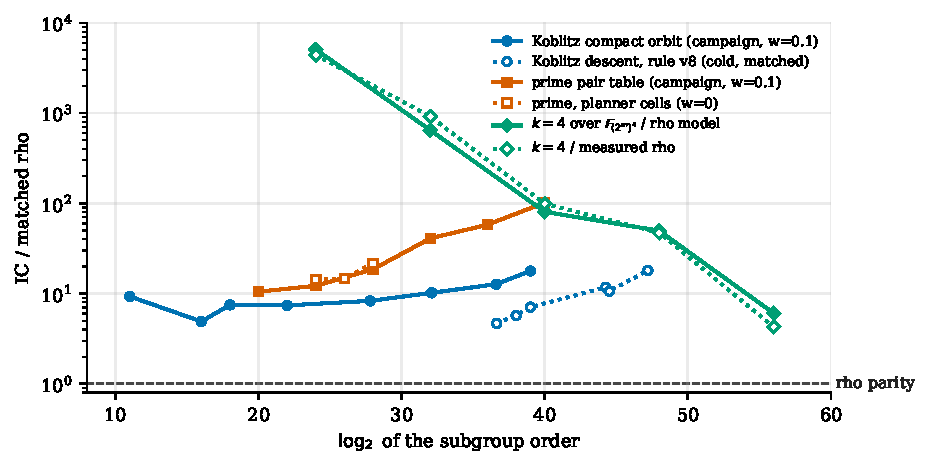
\includegraphics[width=\linewidth]{figures/fig-families.pdf}
\caption[]{Distance to matched rho by family and size. Koblitz and prime
curves: the frontier campaign's priced arms ($w=0.1$, 16 targets $\times$ 2
rounds); open markers are the Koblitz rule at v8 (cold, 64 targets) and the
prime planner cells ($w=0$). $k=4$ over $\FF_{(2^m)^4}$: the characteristic-two
ladder against the negation-map rho model (filled) and a measured rho
(open); the $n\approx2^{56}$ point is one target. Curves and units differ
between families, so the lines are not ranked against each other. Sources:
\art{figures/data-ledger.json}.}
\label{fig:families}
\end{figure}

\section{Koblitz curves}

The leaderboard's Table~A measures a Koblitz descent: aimed $m=3$
collection, then an $m=2$ or $m=3$ descent. It is measured cold on one
unseen public point per process, with 64 points per size, at six sizes
from $2^{36.6}$ to $2^{47.2}$. Figure~\ref{fig:koblitz} shows the rule at
three baselines.
\begin{itemize}
\item \emph{v3 to v7 (same rho).} Index calculus became $1.52$--$1.89\times$
  faster, and the cold ratio fell from $5.23$--$20.97$ to
  $3.43$--$11.5$. The board carries the v7 figures, validated
  (\S\ref{sec:gate}).
\item \emph{v8 (matched rho).} In the same binary, rho's signed-Frobenius
  canonicalisation batched 16 lanes at a time raised the gap by
  $1.30$--$1.58\times$ at every size, to
  \[
    4.67\,[4.34,5.07],\ 5.70,\ 7.07,\ 11.75,\ 10.65,\ 18.07\,[15.98,20.58].
  \]
  All six values lie inside ranges declared before the rows were taken.
  The 408 rows of each run all pass the \texttt{vs\_rho} check
  (\art{research/ic_tool_program/rule/v8/README.md}).
\item \emph{Canonical-step rho (a model).} Pricing rho at the canonical
  batched step gives $6.45$--$23.32\times$ in v8's unit, and
  $9.9$--$43\times$ at rule v4~(\S\ref{sec:ladder3}).
\end{itemize}
The slope of the gap in $\ln r$ is $0.168$ $[0.128,0.208]$ at v8 against
$0.176$ at v3. The v3$\to$v7 improvement lowered the constant, not the
growth.

\begin{figure}[t]
\centering
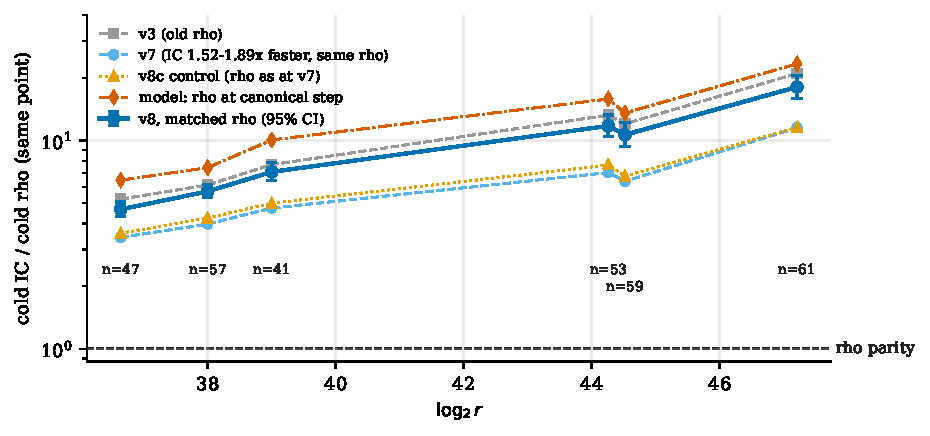
\includegraphics[width=\linewidth]{figures/fig-koblitz-rule.pdf}
\caption[]{The Koblitz rule at three baselines: cold IC over cold rho on the
same public point, 64 targets per size. From v3 to v7 the IC improved
against the same rho. v8 runs the same IC against a matched, faster rho;
its same-binary control, v8c, reproduces v7. The dash-dot line prices rho
at the canonical step. Source:
\art{research/ic_tool_program/rule/v8/README.md}.}
\label{fig:koblitz}
\end{figure}

\paragraph{The priced campaign.} The closest Koblitz arm, compact
Frobenius orbits, is $3.8$--$15\times$ signed-Frobenius rho at $w=0$. Fully
priced against fully priced rho, its best cell is $1.566$ $[0.992,2.347]$;
the ratio is never below 1 and grows as $r^{0.165\,[0.117,0.213]}$.

\paragraph{$n=83$.} The cold pipeline uses the base K1107/root11, which
confirmed a saving of $1.195$\,s $[0.957,1.433]$ on a $115$\,s process (16
public points, GitHub Tier~1 host). The last cold IC/rho ratio is the
K1120 holdout's $55.4$, from five points. A matched precomputed-rho
reproduction on 28 October gave median online IC over rho as follows
(\art{research/n83_k1107_bl_reproduction_20261028/RESULT.md}):
\begin{itemize}
\item $40.9$ $[7.58,141.9]$ against 650\,s table walks;
\item $4.10$ $[1.58,24.8]$ with walks matched to IC set-up;
\item $33.1$ $[6.60,74.4]$ with a table matched to IC memory.
\end{itemize}
Cold, IC took $155.5$\,s against $36.96$\,s for plain rho over all 16
targets. In operation counts the order flips across the pricing band, so
no ranking is made.

\section{Prime curves}

\paragraph{Generic track.} The prime-field programme's owner decisions of
29 October split prime-field index calculus into two counted tracks
(\art{research/prime_ic_program_20261029/DECISIONS.md}):
\begin{itemize}
\item a \emph{generic} track, with table, pair-table and root-finding
  oracles, labelled ``bounded by $\sqrt r$; cannot beat rho'';
\item an \emph{algebraic} track, whose prime baseline is empty.
\end{itemize}
On the generic track:
\begin{itemize}
\item \emph{Table~B} (validated). The prime rows are $5.47$--$13.5\times$
  matched negation rho at 10--24 bits.
\item \emph{Campaign.} The two-summand pair table runs from $10.5\times$
  rho at 20 bits to $101.8\times$ at 40 bits ($w=0.1$). Its fitted
  exponent is $0.620$ $[0.557,0.663]$ against rho's $0.435$, which is the
  $r^{2/3}$ against $r^{1/2}$ of Chapter~\ref{ch:model}.
\item \emph{A $k$-sum table oracle} (28 October,
  \art{research/prime_ksum_table_20261028/}). A negation-folded table of
  every signed 4-sum of a smaller base lowers mean $S$ at $w=0$ by
  $1.9\times$ at 20 bits, rising to $7.2\times$ at 40 bits ($83.7\to11.6$).
  The fitted exponent falls from $0.620$ $[0.586,0.650]$ to $0.521$
  $[0.506,0.538]$, against the theory value $k/(2k-1)=4/7$. That leaves
  $5.3\times$ rho at 20 bits and $13.1\times$ at 40 bits. 2{,}016 runs were
  verified and replayed; the host was L0, and there is no validation.
  The source notes that the method is generic, so its limit is baby-step
  giant-step.
\item \emph{A new 20-bit baseline} (validated,
  \art{research/prime_base_oracle_tuning_20261029/}). Raising the factor
  base from 32 to 45 gives $0.818$ $[0.773,0.866]$ of the incumbent at
  $w=0$. A second host (L2) replayed all 1{,}008 records identically and
  gave $0.836$ $[0.806,0.866]$. The distance to negation rho falls from
  $9.47$ to $7.75$ $[6.92,8.70]$. The same rule at 24 and 28 bits was a
  relabelling, and at 32 bits null.
\item \emph{Planner cells.} These are $12.6$--$25.8\times$ rho.
\end{itemize}

\paragraph{Algebraic track.} The Kummer tower is $28$--$159\times$ rho
(158.9 $[121.6,221.4]$ at 30 bits). No algebraic prime baseline exists.
Its solving degree is the subject of \S\ref{sec:fd-pkm}.

\section{Binary curves of prime degree}

Table~B's random-binary rows are $10.6$--$38.2\times$ matched rho at
$\FF_{2^{15}}$--$\FF_{2^{27}}$, and they are validated. A cofactor-projected
base cuts three of them by $1.29$--$3.36\times$, leaving $6.1$--$14.4\times$.
That base is not yet a board row. For Certicom ECC2-131, the $m=3$ floor
with a free oracle is already above rho~(Chapter~\ref{sec:binary}).

\section{Weak extension-field families}

\begin{figure}[t]
\centering
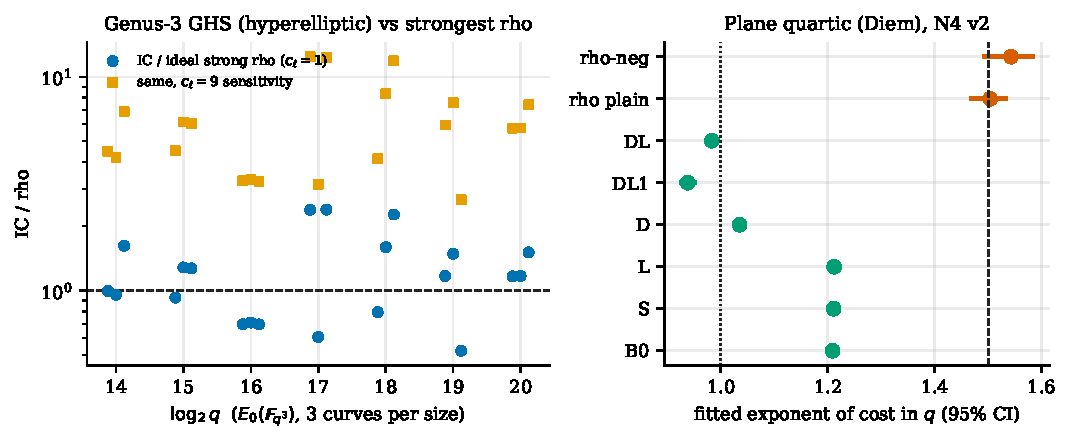
\includegraphics[width=\linewidth]{figures/fig-weak.pdf}
\caption[]{Weak families.
\emph{Left:} genus-3 GHS index calculus (hyperelliptic, double large primes,
round 4) over the ideal strong rho on 21 instances of $E_0(\FF_{q^3})$,
in round 4's unit. Blue: one subgroup multiplication priced at one
$\FF_q$ multiplication, the registered unit. Orange: priced at nine, the
protocol's sensitivity. Below the dashed line IC is cheaper. Source:
\art{research/ghs3_vs_rho_20261023/TABLES.md}.
\emph{Right:} plane-quartic (Diem) index calculus, N4~v2. Fitted exponents
of cold cost in $q$ over $k=8$--$22$ against plain and negation rho, at
$w=0$. Dotted line: $\tilde O(q)$. Dashed line: rho's $q^{3/2}$. Source:
\art{research/quartic_n4v2_20261020/README.md}. Data:
\art{figures/data-new.json}.}
\label{fig:weak}
\end{figure}

Only in these families (Figure~\ref{fig:weak}) does index calculus approach rho or go below it.
\begin{itemize}
\item \emph{Genus 3 via cubic GHS, hyperelliptic route.} This is the
  programme's only preregistered decision of IC below the strongest rho:
  at $q=2^{16}$, IC over the ideal rho reference is $0.70$, $0.71$ and
  $0.70$. At six other sizes the decision is unresolved, and the pooled
  slope is flat ($0.034$ $[-0.047,0.105]$ per bit). Pricing one subgroup
  multiplication at nine $\FF_q$ multiplications puts every instance at
  $2.7$--$12.4\times$ rho (Chapter~\ref{sec:transfer}).
\item \emph{Genus 3 via cubic GHS, plane-quartic route (Diem).} Double
  large primes, structured elimination and Lanczos give a fitted exponent
  of $0.983$ $[0.975,0.993]$ against negation rho's $1.543$. The ratio is
  $0.005$ $[0.004,0.008]$ of negation rho at $q=2{,}097{,}091$, and the
  interpolated crossover is $q^*=555$ $[389,752]$
  (\art{research/quartic_n4v2_20261020/}). The 501 IC units and 2{,}442 rho
  runs are all verified. Three caveats: the host was L0 under heavy load,
  there is no validation file, and the frozen baseline's records do not
  replay. This is a measurement of a known result (Diem, Diem--Thomé).
\item \emph{Joux--Vitse cover of $E(\FF_{p^6})$.} IC is $1.59$--$1.98\times$
  a pooled rho constant at $p=1009$, closing as about $p^{-2}$. This is a
  lower-bound comparison.
\item \emph{$k=4$ over $\FF_{(2^m)^4}$.} IC is $5.2\times$ rho at $m=15$
  after corrections; the crossover is unsupported
  (Chapter~\ref{ch:extension}).
\item \emph{GHS covers over $\FF_{4096}$.} Exact genus-3 covers found by
  search are $549$--$2{,}039\times$ rho in full transfer cost
  (\art{research/ghs_q16_genus3_subcovers_20261028/REPORT.md}).
\end{itemize}

\section{Summary}

\begin{table}[h]
\centering\small
\caption[]{Smallest measured distances to rho, by family.}
\label{tab:nearest}
\begin{tabularx}{\linewidth}{@{}>{\raggedright}p{3.9cm}l>{\raggedright\arraybackslash}X@{}}
\toprule
Family & IC/rho & Qualifier \\
\midrule
Plane quartic via cubic GHS, $q\approx2^{21}$ & $0.005$ & negation rho; weak family; L0; no validation file \\
Genus-3 hyperelliptic via GHS, $q=2^{16}$ & $0.70$ & ideal strong rho; one size of seven; pricing-sensitive \\
Joux--Vitse cover, $p=1009$ & $1.59$--$1.98$ & pooled rho constant; lower bound \\
$k=4$, $\FF_{(2^m)^4}$, $m=15$ & $5.2$ & two targets; crossover unsupported \\
Koblitz, fully priced orbit (best cell) & $1.566$ & never below 1; grows as $r^{0.165}$ \\
Koblitz rule v8, $2^{36.6}$ & $4.67$ & cold, matched, 64 targets \\
Prime, $k$-sum table, 20 bits & $5.3$ & generic track; not validated \\
Prime, Table~B, 12 bits & $5.47$ & validated \\
Random binary, Table~B & $10.6$ & validated \\
Koblitz $n=83$ & $55.4$ & cold, five points \\
\bottomrule
\end{tabularx}
\end{table}

On every prime-order curve of cryptographic shape that the programme
measured, rho is cheaper. Index calculus goes below rho only in weak
extension-field families, which is where theory said it would. There the
programme's contribution is matched, priced, verified measurement of
known algorithms.
